%% LyX 2.3.6.2 created this file.  For more info, see http://www.lyx.org/.
%% Do not edit unless you really know what you are doing.
\documentclass[english]{article}
\usepackage[T1]{fontenc}
\usepackage[utf8]{inputenc}
\usepackage[letterpaper]{geometry}
\geometry{verbose,tmargin=1in,bmargin=1in,lmargin=1in,rmargin=1in}
\usepackage{verbatim}
\usepackage{textcomp}
\usepackage{amsmath}
\usepackage{amsthm}
\usepackage{amssymb}
\usepackage{graphicx}

\makeatletter
%%%%%%%%%%%%%%%%%%%%%%%%%%%%%% Textclass specific LaTeX commands.
\numberwithin{equation}{section}
\numberwithin{figure}{section}

%%%%%%%%%%%%%%%%%%%%%%%%%%%%%% User specified LaTeX commands.
\usepackage{tikz}
\usetikzlibrary{quantikz}
\usetikzlibrary{calc,matrix,fit}
\tikzset{pics/grid/.style={code={\tikzset{wonderich/.cd,#1}
    \def\pv##1{\pgfkeysvalueof{/tikz/wonderich/##1}}%
    \draw[thick] (0.1,0.1) grid (\pv{nx}+0.9,\pv{ny}+0.9);}},
pics/nodes/.style={code={\tikzset{wonderich/.cd,#1}
    \def\pv##1{\pgfkeysvalueof{/tikz/wonderich/##1}}%   
    \path  foreach \X in {1,...,\pv{nx}} {
      foreach \Y in {1,...,\pv{ny}} { 
      (\X,\Y)node[minimum size=\pv{r},style/.expanded=\pv{style},inner sep=0pt]{}} };
}},
wonderich/.cd,nx/.initial=4,ny/.initial=4,r/.initial=4pt,
    style/.initial={circle,fill}}
\usepackage{braket}

\makeatother

\usepackage{babel}
\begin{document}
\title{Tensor Network Contractions for Simulating Quantum Circuits on FPGAs}
\author{Maksim Levental}
\maketitle
\begin{abstract}
Most research in quantum computing today is performed against simulations
of quantum computers rather than true quantum computers. Simulating
a quantum computer entails implementing all of the unitary operators
corresponding to the quantum gates as matrices. For high numbers of
qubits, performing matrix multiplications for these simulations becomes
quite expensive, since $n$-qubit operators correspond to $2^{n}$-dimensional
matrix representations. One way to accelerate such a simulation is
to use field programmable gate array (FPGA) hardware to efficiently
compute the matrix multiplications. Though FPGAs can efficiently perform
matrix multiplications they are memory bound, having relatively small
block random access memory. One way to potentially reduce the memory
footprint of a quantum computing system is to represent it as a tensor
network; tensor networks are a formalism for representing compositions
of tensors wherein economical tensor contractions are readily identified.
Thus we explore tensor networks as a means to reducing the memory
footprint of quantum computing systems and broadly accelerating simulations
of such systems.
\end{abstract}
\global\long\def\twovec#1#2{\begin{pmatrix}#1\\
 #2 
\end{pmatrix}}%

\global\long\def\C{\mathbb{C}}%

\global\long\def\R{\mathbb{R}}%

\global\long\def\bbra#1{\bra{#1}}%

\global\long\def\kket#1{\ket{#1}}%

\tableofcontents{}

\section{Introduction}

Quantum computing (QC) refers to the manipulation and exploitation
of properties of quantum mechanical (QM) systems to perform computation.
QM systems exhibit properties such as superposition and entanglement
and clever \textit{quantum algorithms} transform these systems to
perform general computation. Unsurprisingly, the technique was intially
conceived of as a way to simulate physical systems themselves:
\begin{quotation}
``\ldots{} {[}N{]}ature isn't classical, dammit, and if you want to
make a simulation of nature, you'd better make it quantum mechanical,
and by golly it's a wonderful problem, because it doesn't look so
easy.''
\end{quotation}
This closing \cite{feynman1982simulating} remark from the keynote
at the 1\textsuperscript{st} Physics of Computation Conference in
1981, delivered by the late Richard Feynman, cavalierly, but accurately,
expresses that initial goal of quantum computing. Although modeling
and simulating physical systems on quantum computers remains a thriving
area of research we narrow our focus here to QC as it pertains to
solving general computational problems. Such problems include unstructured
search \cite{10.1145/237814.237866}, integer factorization \cite{365700},
combinatorial optimization \cite{farhi2014quantum}, and many others.
It is conjectured that some quantum algorithms enable quantum computers
to exceed the computational power of classical computers \cite{Zhong1460}.
QC systems are composed of so-called quantum bits, or \textit{qubits},
that encode initial and intermediate states of computations (final
states are the results of measurement and therefore are encoded on
classical bits). Transformations between states are effected by time-reversible
\textit{unitary} \textit{operators.} A formalism for representing
quantum computation is the \textit{quantum circuit} formalism, where
semenatically related collections of $n$ qubits are represented as
\textit{registers} and transformations are represented as gates, connected
to those registers by wires, and applied in sequence.

As already mentioned, in hardware, quantum circuits correspond to
physical systems that readily exhibit quantum mechnical properties;
examples of physical qubits include transmons, ion traps and topological
quantum computers \cite{NAP25196}. Current state of the art QC systems
are termed Noisy Intermediate-Scale Quantum (NISQ) systems. Such systems
are characterized by moderate quantities of physical qubits (50-100)
but relatively few logical qubits (i.e. qubits robust to inteference
and noise). Due to these limitations (and, more broadly, the relative
scarcity of functioning QC systems), most research on quantum algorithms
is performed with the assistance of simulators of QC systems. Such
simulators perform simulations by representing $n$-qubit circuit
as $2^{n}$-dimensional complex vectors and transformations on those
vectors as $2^{n}$-dimensional complex matrix-vector multiplication.
Naturally, due to this exponential growth, naively executing such
simulations quickly become infeasible for $n>50$ qubits \cite{pednault2020paretoefficient},
both due to memory constraints and compute time. 

A field-programmable gate array (FPGA) is a device designed to be
configured by a user into various arrangements of (classical) gates
and memory. FPGAs consist of arrays (hence the name) of configurable
logic blocks (CLBs), block ram (BRAM), and programmable busses that
connect CLBs and RAM into various topologies (see figure \ref{fig:FPGA-floorplan-diagram}).
The CLBs typically contain arithmetic logic units and lookup tables
(LUTs), that can be programmed to represent truth tables for many
boolean functions. Using high-level description languages (such as
VHDL or Verilog) designers specify modules and compose them into circuits
(also known as a \textit{dataflows}) that perform arbitrary computation.
Typically FPGAs run at lower clock speeds (100-300MHz) than either
conventional processors or even graphics processors but nonetheless
they excel at latency constrained computations owing to their fully
``synchronous'' nature (all modules in the same \textit{clock domain}
execute simultaneously).At first glance FPGAs seem like a suitable
platform for performant simulation of quantum systems when runtime
is of the essence. Unfortunately BRAM is one of the more limited resources
on an FPGA and therefore it becomes necessary to explore memory reduction
strategies for simulations (as well as runtime reduction strategies). 

It's the case that matrices are a subclass of a more general mathematical
object called a \textit{tensor} and composition of matrices as \textit{tensor
contraction}.\textit{ Tensor networks} (TNs) are decompositions (i.e.
factorizations) of very high-dimensional tensors into networks (i.e.
graphs) of low-dimensional tensors. TNs have been successfullly employed
in reducing the memory requirements of simulations of QC systems \cite{pednault2020paretoefficient}.
The critical feature of tensor networks that make them useful for
QC is the potential to perform tensor contractions on the smaller
tensors in an order such that, ultimately, the memory and compute
time requirements are lower than for the matrix-vector multiplication
representation. Existing applications of TNs to quantum circuits focus
primarily on memory constraints on general purpose computers \cite{Fried_2018}
and distributed environments \cite{McCaskey_2018}. Hence, we explore
tensor networks as a means of reducing the memory footprint of quantum
circuits with particular attention to dimensions of the designs space
as they pertain to deployment to FPGAs.

The remainder of this report is organized as follows: section \ref{sec:Background}
covers the necessary background wherein subsection \ref{sec:Quantum-Circuits}
very briefly reviews quantum computation and quantum circuits (with
particular focus on aspects that will be relevant for tensor networks
and FPGAs), section \ref{sec:Tensor-Networks} defines tensor networks
fairly rigorously and discusses algorithms for identifying optimal
contraction orders, section \ref{sec:FPGAs} discusses the constraints
imposed by virtue of deploying to FPGA, section \ref{sec:Implementation}
describes our implementation of <TODO>, section \ref{sec:Evaluation}
reports our results on various empirical experiments, and section
\ref{sec:Conclusion} concludes with future research directions.

\section{Background\label{sec:Background}}

\subsection{Quantum Computing\label{sec:Quantum-Circuits}}

We very (very) quickly review quantum computing and quantum circuits
as they pertain to our project. For a much more pedagogically sound
introduction consult \cite{j2020quantum}. As already alluded to,
quantum computing exploits properties of quantum mechanical systems
in order to perform arbitrary computation. The fundamental unit of
quantum computation is a qubit, defined as two-dimensional quantum
system with state vector $\psi$ an element of a Hilbert space\footnote{A Hilbert space $H$ is a vector space augmented with an inner product
such that, with respect to the metric induced by that inner product,
all Cauchy sequences converge.} $H$:
\[
\psi:=\alpha\twovec 10+\beta\twovec 01\equiv\twovec{\alpha}{\beta}
\]
where $\alpha,\beta\in\mathbb{\C}$ and $\left|\alpha\right|^{2}+\left|\beta\right|^{2}=1$.
This exhibits the superposition property of the qubit\footnote{We say that the qubit is in a superposition of the basis vectors/states.}.
Collections of qubits have state vectors that represented by the \textit{tensor
product }of the individual states of each qubit; for example, two
qubits $\psi,\phi$ have state vector
\[
\psi\otimes\phi:=\twovec{\alpha}{\beta}\otimes\twovec{\alpha'}{\beta'}\equiv\begin{pmatrix}\alpha\alpha'\\
\alpha\beta'\\
\beta\alpha'\\
\beta\beta'
\end{pmatrix}
\]
where the second $\otimes$ is the Kronecker product and $\alpha\alpha'$
indicates conventional complex multiplication. Note that the basis
relative to which $\psi\otimes\phi$ is represented is the standard
basis for $\C^{4}$ and thus we observe exponential growth in the
size of the representation of an $n$-qubit system. An alternative
notation for state vectors is Dirac notation:
\[
\psi\equiv\alpha\kket 0+\beta\kket 1
\]
\[
\psi\otimes\phi\equiv\alpha\alpha'\kket{00}+\alpha\beta'\kket{01}+\beta\alpha'\kket{10}+\beta\beta'\kket{11}
\]
Of particular import for QC are the \textit{entangled }or \textit{bell
states}; they correspond to multi-qubit states, such as 
\[
\xi=\frac{1}{\sqrt{2}}\ket{00}+\frac{1}{\sqrt{2}}\ket{11}
\]
that cannot be ``factored'' into component states\footnote{$\xi$ cannot be factored because there is no solution to the set
of equations (for $\alpha,\alpha',\beta,\beta'$)
\[
\alpha\alpha'=\frac{1}{\sqrt{2}},\quad\alpha\beta'=0,\quad\beta\alpha'=0,\quad\beta\beta'=\frac{1}{\sqrt{2}}
\]
}. Then, naturally, changes in qubit states are represented as unitary\footnote{A matrix $U$ is unitary iff $UU^{\dagger}=U^{\dagger}U=I$, i.e.
it is its own Hermitian conjugate or more simply if it is ``self-inverse''.} matrices $U$; for example
\[
\psi'=U\psi=\begin{pmatrix}U_{00} & U_{01}\\
U_{10} & U_{11}
\end{pmatrix}\twovec{\alpha}{\beta}=\twovec{U_{00}\alpha+U_{01}\beta}{U_{10}\alpha+U_{11}\beta}
\]
Matrix representations of transformations on multi-qubit states are
constructed using the Kronecker product on the individual matrix representations;
for example

\[
U\otimes V:=\begin{pmatrix}U_{00}V & U_{01}V\\ U_{10}V & U_{11}V \end{pmatrix}:=\begin{pmatrix}
 U_{00} V_{00} & U_{00} V_{01} & U_{01} V_{00} & U_{01} V_{01} \\
 U_{00} V_{10} & U_{00} V_{11} & U_{01} V_{10} & U_{01} V_{11} \\
 U_{10} V_{00} & U_{10} V_{01} & U_{11} V_{00} & U_{11} V_{01} \\
 U_{10} V_{10} & U_{10} V_{11} & U_{11} V_{10} & U_{11} V_{11}
\end{pmatrix}
\]Here we see again an exponential growth in representation size as
a function of number of qubits. 

\begin{figure}
\begin{quantikz}
%\gategroup[wires=3,steps=11]{}
&\lstick{$|{0}\rangle$} & \gate{H}&\ctrl{1} & \ctrl{2} &\qw &\qw 
 \rstick[wires=3]{$\frac{|{000}\rangle + |{111}\rangle}{\sqrt{2}}$} 
\\
&\lstick{$|{0}\rangle$} & \gate{H}& \control{} & \qw& \gate{H} &\qw
\\
&\lstick{$|{0}\rangle$} & \gate{H}& \qw & \control{} & \gate{H} &\qw
&&&&
\end{quantikz}
\centering{}\caption{Quantum Circuit representing 3-qubit entanglement effected by application
of success Hadamard gates.\label{fig:Quantum-Circuit-representing-1}}
\end{figure}

As already alluded to, quantum circuits are a formalism for representing
quantum computation in general and algorithms designed for quantum
computers in particular. In the quantum circuit formalism qubit states
are represented by wires and unitary transformations are represented
by gates (see figure \ref{fig:Quantum-Circuit-representing-1}), much
like classical combinational logic circuits might be, though, whereas
combinational logic is ``memoryless''\footnote{The output of a combinational logic circuit at any time is only a
function of the elements of the circuit and its inputs.}, sequences of quantum gates specified by a quantum circuit do in
fact connote the evolution (in time) of the qubits. In addition quantum
gates, as opposed to classical gates, are necessarily reversible and
hence there are no quantum analogs to some classical gates such as
NOT and OR.

\subsection{Tensor Networks\label{sec:Tensor-Networks}}

We quickly define tensors and and then move on to tensor network methods.

\subsubsection{Definition}

One definition of a tensor\footnote{There are several more at varying levels of mathematical sophistication.
Chapter 14 of \cite{roman2007advanced} is the standard reference.
Ironically, it is this author's opinion that one should shy away from
physics oriented expositions on tensors.} $T$ is as an element of a tensor product space\footnote{The collection of tensor products of elements of the component spaces
quotiented by an equivalence relation.}:
\[
T\in\underbrace{V\otimes\cdots\otimes V}_{p{\text{ copies}}}\otimes\underbrace{V^{*}\otimes\cdots\otimes V^{*}}_{q{\text{ copies}}}
\]
where $V^{*}$ is dual\footnote{The dual space to a vector space $V$ is the vector $V^{*}$ consisting
of linear maps $f:V\rightarrow\R$. The dual basis of the dual space
consists of $f_{i}$ such that $f_{i}\left(\mathbf{e}_{i}\right)=\delta_{ij}$.
It is convention to write $f_{i}$ as $\mathbf{e}^{i}$ (note the
superscript index).} to $V$. Then $T$, in effect, acts a multilinear map
\[
{\displaystyle T:\underbrace{V^{*}\times\dots\times V^{*}}_{p{\text{ copies}}}\times\underbrace{V\times\dots\times V}_{q{\text{ copies}}}\rightarrow\R}
\]
by ``applying'' $p$ elements from $V$ to $p$ elements of $V^{*}$
and $q$ elements from $V^{*}$ to $q$ elements of $V$. Note the
swapping of the orders of $V,V^{*}$ in both the definitions and the
description. $T$'s coordinate basis representation

\begin{equation}
{\displaystyle T\equiv T_{j_{1}\dots j_{q}}^{i_{1}\dots i_{p}}\;\mathbf{e}_{i_{1}}\otimes\cdots\otimes\mathbf{e}_{i_{p}}\otimes\mathbf{e}^{j_{1}}\otimes\cdots\otimes\mathbf{e}^{j_{q}}}\label{eq:tensor_coord}
\end{equation}
is determined by its evaluation on each set of bases

\[
{\displaystyle T_{j_{1}\dots j_{q}}^{i_{1}\dots i_{p}}:=T\left(\mathbf{e}^{i_{1}},\ldots,\mathbf{e}^{i_{p}},\mathbf{e}_{j_{1}},\ldots,\mathbf{e}_{j_{q}}\right)}
\]
The pair $\left(p,q\right)$ is called the \textit{type }or\textit{
valence} of \textbf{$T$} while $\left(p+q\right)$ is the \textit{order}
of the tensor. \textbf{Note that we do not use rank to mean either
of these things}. Note further that eqn. \ref{eq:tensor_coord} in
fact represents a linear sum of basis elements, as it employs Einstein
summation convention\footnote{Repeated indices in juxtapose position indicate summation $a_{i}b^{i}:=\sum_{i}a[i]b[i]$.}. 

There are two important operations on tensors we need to define. Firstly,
we can form the tensor product $Z$ of two tensors $T,W$, of types
$\left(p,q\right),\left(r,s\right)$ respectively, to obtain a tensor
of type $\left(p+r,q+s\right)$:
\begin{align*}
Z & :=T\otimes W\\
 & \;=\left(T_{j_{1}\dots j_{q}}^{i_{1}\dots i_{p}}\;\mathbf{e}_{i_{1}}\otimes\cdots\otimes\mathbf{e}_{i_{p}}\otimes{\mathbf{e}}^{j_{1}}\otimes\cdots\otimes{\mathbf{e}}^{j_{q}}\right)\otimes\left(W_{l_{1}\dots l_{s}}^{k_{1}\dots k_{r}}\;\mathbf{e}_{k_{1}}\otimes\cdots\otimes\mathbf{e}_{k_{r}}\otimes{\mathbf{e}}^{l_{1}}\otimes\cdots\otimes{\mathbf{e}}^{l_{s}}\right)\\
 & \;=\left(T_{j_{1}\dots j_{q}}^{i_{1}\dots i_{p}}W_{l_{1}\dots l_{s}}^{k_{1}\dots k_{r}}\;\mathbf{e}_{i_{1}}\otimes\cdots\otimes\mathbf{e}_{i_{p}}\otimes\mathbf{e}_{k_{1}}\otimes\cdots\otimes\mathbf{e}_{k_{r}}\otimes{\mathbf{e}}^{j_{1}}\otimes\cdots\otimes{\mathbf{e}}^{j_{q}}\otimes{\mathbf{e}}^{l_{1}}\otimes\cdots\otimes{\mathbf{e}}^{l_{s}}\right)\\
 & :=Z_{j_{1}\dots j_{q+s}}^{i_{1}\dots i_{p+r}}\;\mathbf{e}_{i_{1}}\otimes\cdots\otimes\mathbf{e}_{i_{p+r}}\otimes{\mathbf{e}}^{j_{1}}\otimes\cdots\otimes{\mathbf{e}}^{j_{q+s}}
\end{align*}
\begin{comment}
The attentive reader should notice that the coordinate representation
of two tensors is 
\end{comment}
Despite it being obvious, its important to note that the tensor product
$Z$ produces a tensor of order $\left(p+r+q+s\right)$, i.e. higher
than either of the operands. On the contrary, \textit{tensor contraction}
reduces the order of a tensor. We define the contraction $Y$ of type
$\left(a,b\right)$ of a tensor $T$ to be the ``pairing'' of the
$a$th and $b$th bases: 
\begin{align*}
Y & :=T_{j_{1}\dots j_{q}}^{i_{1}\dots i_{p}}\;\mathbf{e}_{i_{1}}\otimes\cdots\left[\mathbf{e}_{i_{a}}\right]\cdots\otimes\mathbf{e}_{i_{p}}\otimes\left(\mathbf{e}_{i_{a}}\cdot\mathbf{e}^{j_{b}}\right)\otimes\mathbf{e}^{j_{1}}\otimes\cdots\left[\mathbf{e}^{j_{b}}\right]\cdots\otimes\mathbf{e}^{j_{q}}\\
 & \;=T_{j_{1}\dots j_{q}}^{i_{1}\dots i_{p}}\delta_{i_{a}}^{j_{b}}\;\mathbf{e}_{i_{1}}\otimes\cdots\left[\mathbf{e}_{i_{a}}\right]\cdots\otimes\mathbf{e}_{i_{p}}\otimes\mathbf{e}^{j_{1}}\otimes\cdots\left[\mathbf{e}^{j_{b}}\right]\cdots\otimes\mathbf{e}^{j_{q}}\qquad\left(\text{since }\mathbf{e}_{i}\cdot\mathbf{e}^{j}=\delta_{i}^{j}\right)\\
 & \;=\left(\sum_{j_{b}}T_{j_{1}\dots j_{b}\dots j_{q}}^{i_{1}\dots j_{b}\dots i_{p}}\right)\;\mathbf{e}_{i_{1}}\otimes\cdots\left[\mathbf{e}_{i_{a}}\right]\cdots\otimes\mathbf{e}_{i_{p}}\otimes\mathbf{e}^{j_{1}}\otimes\cdots\left[\mathbf{e}^{j_{b}}\right]\cdots\otimes\mathbf{e}^{j_{q}}\\
 & :=Y_{j_{1}\dots\left[j_{b}\right]\dots j_{q}}^{i_{1}\dots\left[i_{a}\right]\dots i_{p}}\;\mathbf{e}_{i_{1}}\otimes\cdots\left[\mathbf{e}_{i_{a}}\right]\cdots\otimes\mathbf{e}_{i_{p}}\otimes\mathbf{e}^{j_{1}}\otimes\cdots\left[\mathbf{e}^{j_{b}}\right]\cdots\otimes\mathbf{e}^{j_{q}}
\end{align*}
where $\left(\cdot\right)$ means inner product and $\left[\cdot\right]$
means omission from sequence. Notice that the order of $Y$ is $\left(p-1,q-1\right)$.
Finally notice that we can omit writing out bases and just manipulate
coordinates. We shall do as such when it simplifies presentation.

As mentioned in the introduction, matrices can be represented as tensors;
for example, the two dimensional $n\times n$ matrix $M$ is taken
to be a tensor of type $\left(1,1\right)$ with basis representation
\[
{\displaystyle M\equiv M_{j}^{i}\;\mathbf{e}_{i}\otimes\mathbf{e}^{j}}
\]
where upper indices correspond to the row index and lower indices
correspond to the column index of the conventional matrix representation
and both range from $1$ to $n$. The attentive reader will notice
that the coordinate representation of the tensor product for type
$\left(1,1\right)$ tensors is exactly the Kronecker product for matrices.
Similarly, tensor contraction for type $\left(1,1\right)$ tensors
is the familiar matrix trace:

\[
M_{j}^{i}\left(\mathbf{e}_{i}\cdot\mathbf{e}^{j}\right)=M_{j}^{i}\delta_{i}^{j}=\sum_{i}M_{i}^{i}
\]
More usefully, we can express matrix-vector multiplication in terms
of tensor contraction; let\textit{ 
\[
\mathbf{x}:=\twovec{x^{1}}{x^{2}}\equiv x^{1}\mathbf{e}_{1}+x^{2}\mathbf{e}_{2}\equiv x^{i}\mathbf{e}_{i}
\]
}where we switch to valence index notation in the column vector for
closer affinity with tensor notation. Then it must be the case that
\[
\mathbf{y}=M\mathbf{x}=\left(M_{j}^{i}\mathbf{e}_{i}\otimes\mathbf{e}^{j}\right)\left(x^{k}\mathbf{e}_{k}\right)=\left(M_{j}^{i}x^{k}\mathbf{e}_{i}\right)\left(\mathbf{e}^{j}\cdot\mathbf{e}_{k}\right)=M_{j}^{i}x^{k}\delta_{k}^{j}\mathbf{e}_{i}=M_{j}^{i}x^{j}\mathbf{e}_{i}
\]
Letting $y^{i}:=M_{j}^{i}x^{j}$ we recognize conventional matrix-vector
multiplication. Employing tensor contraction in this way extends to
matrix-matrix multiplication (and tensor composition more broadly);
for two type $\left(1,1\right)$ tensors $M,N$ we can form the type
$\left(1,1\right)$ tensor $Z$ corresponding to matrix product $M\cdot N$
of $n\times n$ by first taking the tensor product

\[
Z_{lj}^{ik}:=M_{l}^{i}N_{j}^{k}
\]
and then contracting along the off diagonal
\[
Z_{j}^{i}:=Z_{kj}^{ik}=M_{k}^{i}N_{j}^{k}\equiv\sum_{k=1}^{n}M_{k}^{i}N_{j}^{k}
\]
One can confirm that this is indeed conventional matrix multipliation
of two $n\times n$ matrices.

\subsubsection{Tensor Networks}

\begin{figure}
\centering{}    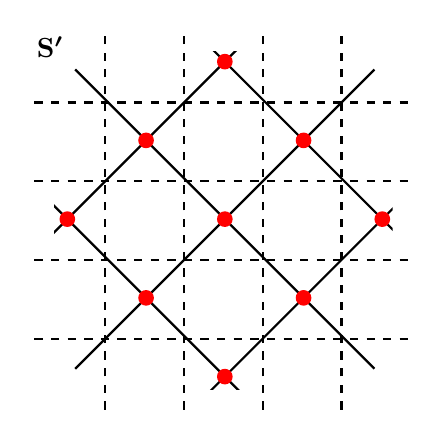
\begin{tikzpicture}
     \draw[dashed]  pic{grid}
     (0.3,4.7) node{$\mathbf{S}\boldsymbol{'}$};
     \clip (0.35,0.35) rectangle (4.65,4.65);
     \path[rotate around={45:(45:2.5)},scale={sqrt(2)},
        shift={(0,-0.75)},transform shape]  pic{grid={nx=3,ny=3}}
        pic[red]{nodes={r=4pt,nx=3,ny=3}};
    \end{tikzpicture}\caption{Projected Entangled Pair State (PEPS) for a 3 \texttimes{} 3 lattice
with open boundary conditions.\label{fig:Projected-Entangled-Pair}}
\end{figure}


\subsection{FPGAs\label{sec:FPGAs}}

FPGAs consist of arrays (hence the name) of configurable logic blocks
(CLBs), block ram (BRAM), and programmable busses that connect CLBs
and RAM into various topologies (see figure \ref{fig:FPGA-floorplan-diagram}).

\begin{figure}
\centering{}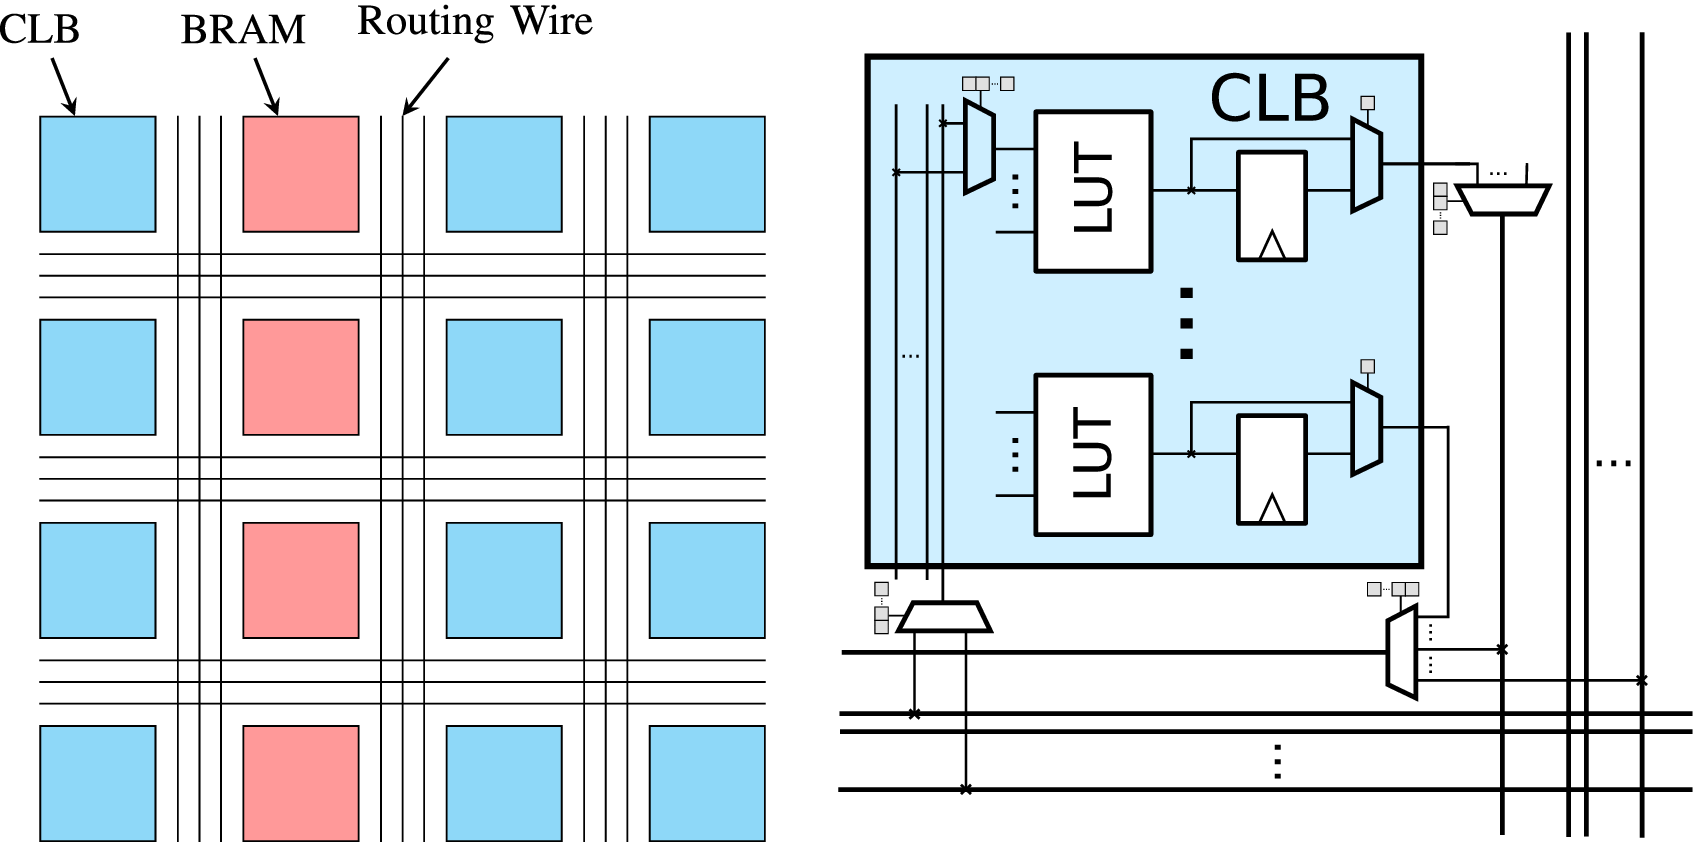
\includegraphics[width=0.5\textwidth]{murra1-2998435}\caption{FPGA floorplan diagram \cite{9103284}.\label{fig:FPGA-floorplan-diagram}}
\end{figure}


\section{Implementation\label{sec:Implementation}}

asdsd

\section{Evaluation\label{sec:Evaluation}}

assd

\section{Conclusion\label{sec:Conclusion}}

\bibliographystyle{plain}
\addcontentsline{toc}{section}{\refname}\nocite{*}
\bibliography{biblio}

\end{document}
